\tikzset{every picture/.style={line width=0.75pt}} %set default line width to 0.75pt        

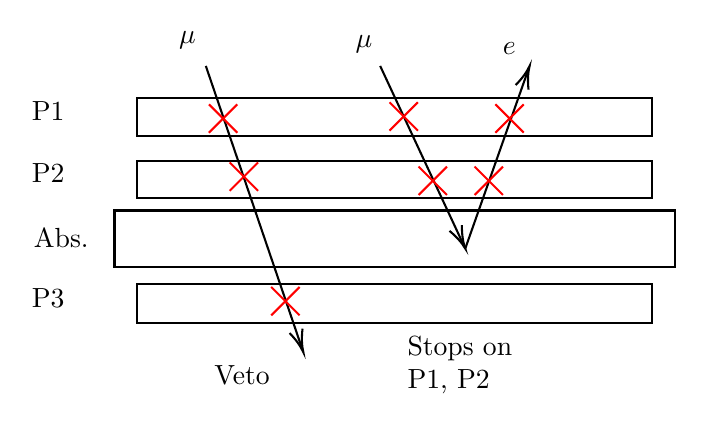
\begin{tikzpicture}[x=0.75pt,y=0.75pt,yscale=-1,xscale=1]
%uncomment if require: \path (0,239); %set diagram left start at 0, and has height of 239

%Shape: Rectangle [id:dp779608831693803] 
\draw   (131,81) -- (379.33,81) -- (379.33,99) -- (131,99) -- cycle ;
%Shape: Rectangle [id:dp6210994436881714] 
\draw   (131,170.33) -- (379.33,170.33) -- (379.33,189) -- (131,189) -- cycle ;
%Shape: Rectangle [id:dp18252585112175712] 
\draw   (120.33,135) -- (390.33,135) -- (390.33,162) -- (120.33,162) -- cycle ;
%Shape: Rectangle [id:dp9173904155089121] 
\draw   (131,111) -- (379.33,111) -- (379.33,129) -- (131,129) -- cycle ;
%Straight Lines [id:da7511843328220018] 
\draw    (164.33,65.33) -- (210.69,201.44) ;
\draw [shift={(211.33,203.33)}, rotate = 251.19] [color={rgb, 255:red, 0; green, 0; blue, 0 }  ][line width=0.75]    (10.93,-3.29) .. controls (6.95,-1.4) and (3.31,-0.3) .. (0,0) .. controls (3.31,0.3) and (6.95,1.4) .. (10.93,3.29)   ;
%Straight Lines [id:da650554014246816] 
\draw    (248.33,65.33) -- (288.49,151.52) ;
\draw [shift={(289.33,153.33)}, rotate = 245.02] [color={rgb, 255:red, 0; green, 0; blue, 0 }  ][line width=0.75]    (10.93,-3.29) .. controls (6.95,-1.4) and (3.31,-0.3) .. (0,0) .. controls (3.31,0.3) and (6.95,1.4) .. (10.93,3.29)   ;
%Straight Lines [id:da9118596186922334] 
\draw    (289.33,153.33) -- (319.67,67.22) ;
\draw [shift={(320.33,65.33)}, rotate = 109.41] [color={rgb, 255:red, 0; green, 0; blue, 0 }  ][line width=0.75]    (10.93,-3.29) .. controls (6.95,-1.4) and (3.31,-0.3) .. (0,0) .. controls (3.31,0.3) and (6.95,1.4) .. (10.93,3.29)   ;
\draw  [color={rgb, 255:red, 255; green, 0; blue, 0 }  ,draw opacity=1 ] (165.83,83.83) -- (179.5,97.5)(179.5,83.83) -- (165.83,97.5) ;
\draw  [color={rgb, 255:red, 255; green, 0; blue, 0 }  ,draw opacity=1 ] (175.83,111.83) -- (189.5,125.5)(189.5,111.83) -- (175.83,125.5) ;
\draw  [color={rgb, 255:red, 255; green, 0; blue, 0 }  ,draw opacity=1 ] (195.83,171.83) -- (209.5,185.5)(209.5,171.83) -- (195.83,185.5) ;
\draw  [color={rgb, 255:red, 255; green, 0; blue, 0 }  ,draw opacity=1 ] (252.83,82.83) -- (266.5,96.5)(266.5,82.83) -- (252.83,96.5) ;
\draw  [color={rgb, 255:red, 255; green, 0; blue, 0 }  ,draw opacity=1 ] (266.83,113.83) -- (280.5,127.5)(280.5,113.83) -- (266.83,127.5) ;
\draw  [color={rgb, 255:red, 255; green, 0; blue, 0 }  ,draw opacity=1 ] (303.83,83.83) -- (317.5,97.5)(317.5,83.83) -- (303.83,97.5) ;
\draw  [color={rgb, 255:red, 255; green, 0; blue, 0 }  ,draw opacity=1 ] (293.83,113.83) -- (307.5,127.5)(307.5,113.83) -- (293.83,127.5) ;

% Text Node
\draw (79,81) node [anchor=north west][inner sep=0.75pt]   [align=left] {P1};
% Text Node
\draw (79,111) node [anchor=north west][inner sep=0.75pt]   [align=left] {P2};
% Text Node
\draw (79,171) node [anchor=north west][inner sep=0.75pt]   [align=left] {P3};
% Text Node
\draw (80,142) node [anchor=north west][inner sep=0.75pt]   [align=left] {Abs.};
% Text Node
\draw (167,208) node [anchor=north west][inner sep=0.75pt]   [align=left] {Veto};
% Text Node
\draw (150,47.4) node [anchor=north west][inner sep=0.75pt]    {$\mu $};
% Text Node
\draw (235,49.4) node [anchor=north west][inner sep=0.75pt]    {$\mu $};
% Text Node
\draw (306,52.4) node [anchor=north west][inner sep=0.75pt]    {$e$};
% Text Node
\draw (260,194) node [anchor=north west][inner sep=0.75pt]   [align=left] {Stops on\\ P1, P2};


\end{tikzpicture}